\documentclass[11pt, letterpaper]{article}
\usepackage[utf8]{inputenc}

\makeatletter
\newcommand{\@BIBLABEL}{\@emptybiblabel}
\newcommand{\@emptybiblabel}[1]{}
\newcommand*{\permcomb}[4][0mu]{{{}^{#3}\mkern#1#2_{#4}}}
\newcommand{\perm}[1][-3mu]{\permcomb[#1]{P}}
\makeatother
\usepackage[hidelinks]{hyperref}
\usepackage{comment}
\usepackage{enumitem}
\usepackage{fullpage}
\usepackage[english]{babel}
\usepackage{graphicx}
\usepackage[colorinlistoftodos]{todonotes}
\usepackage[linesnumbered]{algorithm2e}
\usepackage{tabularx}
\usepackage{diagbox}
\usepackage{caption}
\usepackage{url}
\usepackage{hyperref}
\hypersetup{colorlinks=true}
\usepackage[margin=0.7in]{geometry}    % For reducing margin
\usepackage[english]{babel}
\usepackage{mathtools}
\usepackage{booktabs}
\usepackage{physics}
\usepackage{amsmath,amssymb,amsthm}
\usepackage{fullpage}
\usepackage{enumitem}
\usepackage{tcolorbox}
\usepackage{comment}
\usepackage{framed}

\newcommand{\wx}[1]{\textcolor{magenta}{\bf\small [#1 --WX]}}

\begin{document}

\title{CS 7650: Natural Language Processing \\ Fall 2022 \\ Problem Set 2}
\author{Instructor: Dr. Wei Xu \\ TAs: Chase Perry, Rahul Katre, Rucha Sathe, Xurui Zhang \\Piazza: \url{https://piazza.com/class/l6vgipz0vsm1kk}
\\Gradescope: \url{https://gradescope.com/courses/418978}}
\date{Due: Friday, October 7, 11:59 PM ET}
\maketitle

\section{Understanding Word2Vec}
Given a sequence of words $w_{1}, \ldots, w_{T}$ and context size $c$, the training objective of skip-gram is:
$$
\mathcal{L}=-\frac{1}{T} \sum_{t=1}^{T} \sum_{-c \leq j \leq c, j \neq 0} \log P\left(w_{t+j} \mid w_{t}\right)
$$
where $P\left(w_{o} \mid w_{t}\right)$ is defined as:
$$
P\left(w_{o} \mid w_{t}\right)=\frac{\exp \left(\mathbf{u}_{w_{t}}^{\top} \mathbf{v}_{w_{o}}\right)}{\sum_{k \in V} \exp \left(\mathbf{u}_{w_{t}}^{\top} \mathbf{v}_{k}\right)}
$$
where $\mathbf{u}_{k}$ represents the ``target" vector and $\mathbf{v}_{k}$ represents the``context" vector, for every $k \in V$.\\

\begin{enumerate}[label=(\alph*)]

\item (\textbf{3 pts}) Derive the following gradient (probability w.r.t context vector):
$$
-\frac{\partial \log P\left(w_{o} \mid w_{t}\right)}{\partial \mathbf{v}_{w_{o}}}
$$

\item (\textbf{2 pts}) Imagine that we train the model on a large corpus (e.g. English Wikipedia). Describe the effects of context size $c$ to the resulting word vectors $\mathbf{u}_{w}$, i.e. what if we use context size $c=1,5$, or $100 ?$\\\\

\end{enumerate}
    
\section{Hidden Markov Models and the Viterbi Algorithm}
    We have a toy language with 2 words - “cool” and “shade”. We want to tag the parts of speech in a test corpus in this toy language. There are only 2 parts of speech — NN (noun) and VB (verb) in this language. We have a corpus of text in which we the following distribution of the 2 words:
    
    \begin{table}[h!]
    \centering
    \small
    \begin{tabular}{|l | c | c |}
    \hline & NN & VB\\
    \hline
    cool & 3 & 6 \\
    shade & 7 & 4\\
    \hline
    \end{tabular}
    \end{table}
    Assume that we have an HMM model with the following transition probabilities (* is a special start of the sentence symbol).
    
    \begin{figure}[h]
    \centering
    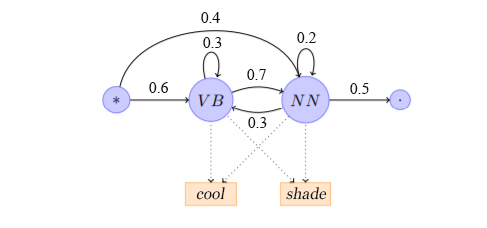
\includegraphics{images/HMM.jpg}
    \caption{HMM model for POS tagging in our toy language.}
    \end{figure}

\begin{enumerate}[label=(\alph*)]

\item (\textbf{2 pts}) Compute the emission probabilities for each word given each POS tag.\\

\item (\textbf{3 pts}) Draw the Viterbi trellis for the sequence “cool shade.”. Highlight the most likely sequence. \href{https://web.stanford.edu/~jurafsky/slp3/A.pdf#page=8}{\color{blue}{Here}} is an  example of Viterbi trellis.

\end{enumerate}

    

\section{LSTMs}


The update equations for a LSTM at timestep $i$ are given in the following equations. Eisenstein Chapter 6.3 may be useful in answering this question. 

\begin{align*} 
    \mathbf{f_i} &= \sigma(\mathbf{W}^{(f)} \mathbf{h_{i-1}} + \mathbf{U}^{(f)} \mathbf{x_{i}}    + \mathbf{B}^{(f)} ) \qquad   &\text{Forget gate} \\
    \mathbf{i_i} &= \sigma(\mathbf{W}^{(i)} \mathbf{h_{i-1}} + \mathbf{U}^{(i)} \mathbf{x_{i}}   + \mathbf{B}^{(i)} ) \qquad  &\text{Input gate} \\
    \mathbf{g_i} &= tanh(\mathbf{W}^{(g)} \mathbf{h_{i-1}} + \mathbf{U}^{(g)} \mathbf{x_{i}} )  \qquad   &\text{Update candidate}\\
    \mathbf{c_i} &= \mathbf{f_i} \odot \mathbf{c}_{i-1}  + \mathbf{i_i} \odot \mathbf{g_i}  \qquad   &\text{Memory cell update}\\
    \mathbf{o_i} &= \sigma(\mathbf{W}^{(o)} \mathbf{h_{i-1}} + \mathbf{U}^{(o)} \mathbf{x_{i}}   + \mathbf{B}^{(o)} ) \qquad   &\text{Output gate}\\
    \mathbf{h_i} &= \mathbf{o_i} \cdot \text{tanh}(\mathbf{c_i})  \qquad   &\text{Output} 
\end{align*} 



\begin{enumerate}[label=(\alph*)]

\begin{table}[h]
    \centering
    \begin{tabular}{|cc|}
    \toprule
    \textbf{Weight} & \textbf{Value} \\
    \midrule
    $\mathbf{W}^{(f)}$ & $[1,-2,-3]$ \\
    $\mathbf{U}^{(f)}$ & $[0,-1,-2]$ \\
    $\mathbf{B}^{(f)}$ & $0$ \\
    $\mathbf{W}^{(i)}$ & $[0,0,1]$\\
    $\mathbf{U}^{(i)}$ & $[-1,-2,-2]$\\
    $\mathbf{B}^{(i)}$ & $1$ \\
    $\mathbf{W}^{(g)}$ & $\begin{bmatrix}
    0 & 1 & -3\\
    -3 & 1 & 0\\
    -2 & -1 & -3
        \end{bmatrix}$ \\
    $\mathbf{U}^{(g)}$ & $\begin{bmatrix}
    1 & 0 & 0 \\
    -2 & -3 & 0\\
    1 & -1 & -2 \end{bmatrix}$ \\
    $\mathbf{W}^{(o)}$ & $[1,0,1]$\\
    $\mathbf{U}^{(o)}$ & $[-1,0,1]$\\
    $\mathbf{B}^{(o)}$ & $-1$ \\
    \bottomrule
    \end{tabular}
    \caption{Weights for LSTM.}
    \label{tab:lstm_weights}
\end{table}

\item (\textbf{1 pt}) In \autoref{tab:lstm_weights} we provide weight values and in \autoref{tab:lstm_intvars} timestep inputs. We'll now compute the value of $\boldsymbol{h}_{i}$ using \autoref{tab:lstm_weights} and \autoref{tab:lstm_intvars}: 

\begin{table}[h!]
    \centering
    \begin{tabular}{|cc|}
    \toprule
    \textbf{Vector} & \textbf{Value} \\
    \midrule
    $\boldsymbol{h}_{i-1}$ & $[3,1,-1]^T$ \\
    $\boldsymbol{c}_{i-1}$ & $[1,0,-4]^T$ \\
    $\boldsymbol{x}_{i}$ & $[-3,-2,-1]^T$ \\
    \bottomrule
    \end{tabular}
    \caption{Input/intermediate variables for LSTM.}
    \label{tab:lstm_intvars}
\end{table}


$\boldsymbol{f}_{i} = \sigma(4 + 4 + 0) = 1.0$ \\
\indent $\boldsymbol{i}_{i} = \sigma(-1 + 9 + 1) = 1.0$ \\
\indent $\boldsymbol{g}_{i} = \text{tanh}([4, -8, -4]^T + [-3, 12, 1]^T) = \text{tanh}([1,4,-3]^T) = [0.76, 1.0, -1.0]^T$\\
\indent $\boldsymbol{c}_{i} = 1.0 \odot [1,0,-4]^T + 1.0 \odot [0.76, 1.0, -1.0]^T = [1.76, 1.0, -5.0]^T $ \\
\indent $\boldsymbol{o}_{i} = \sigma(2 + 2 - 1) = 1.0$\\
\indent $\boldsymbol{h}_{i} = 1.0 \odot \text{tanh}([1.76, 1.0, -5.0]^T) = \mathbf{[0.94, 0.76, -1.0]^T}$\\

The gates of this LSTM do not restrict the flow of any information. To effectively turn this LSTM into an Elman RNN at the current timestep, i.e., include \textbf{only} information from the current input and prior hidden state and \textbf{no} information from the prior memory cell in $\boldsymbol{h}_{i}$, describe the values that you would need to set the gates $\boldsymbol{f}_{i}, \boldsymbol{i}_{i}$ and $\boldsymbol{o}_{i}$ equal to. Only the values for these gates are necessary, do not change the equations for the update.

\item (\textbf{1 pt})  Which variable from the list of intermediate variables in the given equations most closely resembles the hidden state of a standard Elman RNN? (Answer choices are $\boldsymbol{f}_{i}$, $\boldsymbol{i}_{i}$, $\boldsymbol{g}_{i}$, $\boldsymbol{c}_{i}$, $\boldsymbol{o}_{i}$, $\boldsymbol{h}_{i}$).

\item (\textbf{2 pts})  In this problem, all the LSTM gates are scalars. What changes would have to be made to \autoref{tab:lstm_weights} in order to create vector gates? (Specify which weights would change and what their new dimensions would be). What is the benefit of vector gates over scalars?

\item (\textbf{2 pts})   What two problems in RNNs does the inclusion of the memory cell $\boldsymbol{c}_{i}$ improve? What property of its computation allows it to do this?

\end{enumerate}

\section{Conditional Random Fields}
Consider a sequential CRF,
        $$
        \mathrm P(\mathbf{y}|\mathbf{x}) = \frac{1}{Z}\prod_{i=2}^N \exp(\phi_t(y_{i-1}, y_i))\prod_{i=1}^N\exp(\phi_e(y_i, i, \mathbf{x}))
        $$
        $$
        L(\mathbf{x}, \mathbf{y})  = \log \mathrm P(\mathbf{y}|\mathbf{x}) = \sum_{i=2}^N \phi_t(y_{i-1}, y_i) + \sum_{i=1}^N\phi_e(y_i, i, \mathbf{x}) - \log Z
        $$
        In order to compute the loss function, we need two parts, $\sum_{i=2}^N \phi_t(y_{i-1}, y_i) + \sum_{i=1}^N\phi_e(y_i, i, \mathbf{x})$ which is called the gold score (unnormalized conditional log-probability), and $\log Z$.

        \begin{enumerate}[label=(\alph*)]
        
        \item (\textbf{2 pts}) Now we are applying CRF to POS-tagging. The sentence, transition scores and emission scores are shown below. What is the gold score (unnormalized conditional log-probability) of this sentence? Show your work.

        \begin{table}[h!]
        \centering
        \begin{tabular}{lccccccc}
        Sentence: & -START- & Atlanta & is & a   & beautiful & city & -END- \\
        POS tags:  & START   & n       & v  & det & adj       & n    & END  
        \end{tabular}
        \end{table}

        \begin{table}[h!]
        \centering
        \begin{tabular}{|c|c|c|c|c|c|c|}
        \hline
        \diagbox[]{$y_{i-1}$}{$y_i$}      & START & n     & v     & det   & adj   & END   \\ \hline
        START & -0.1  & 0.63  & 0.67  & -1.43 & -1.96 & -0.5  \\ \hline
        n     & -0.9  & 1.24  & 0.76  & 0.41  & 0.23  & 0.65  \\ \hline
        v     & -1.42 & -0.24 & -1.35 & 1.62  & -1.76 & 1.28  \\ \hline
        det   & -1.7  & 0.75  & -0.65 & -0.38 & 1.37  & -1.93 \\ \hline
        adj   & -1.76 & 1.66  & 0.04  & -1.64 & 1.95  & 1.79  \\ \hline
        END   & -1.55 & -0.31 & -1.46 & -0.75 & 0.49  & -1.35 \\ \hline
        \end{tabular}
        \caption*{Transition Scores: $\phi_t(y_{i-1}, y_i)$}
        \end{table}
        
        \begin{table}[h!]
        \centering
        \begin{tabular}{|c|c|c|c|c|c|c|}
        \hline
        \diagbox[]{$x_i$}{$y_i$}          & START & n     & v     & det   & adj   & END   \\ \hline
        -START-   & 1.97  & -4.49 & -3.29 & 3.16  & -0.99 & -0.81 \\ \hline
        Atlanta   & 0.96  & -0.23 & -1.15 & -4.7  & 2.26  & 4.67  \\ \hline
        is        & 4.76  & 1.64  & -1.44 & -1.37 & 1.9   & 1.74  \\ \hline
        a         & -3.86 & -2.65 & -1.37 & 0.11  & 3.1   & 0     \\ \hline
        beautiful & -4.72 & 3.23  & -0.7  & 0.19  & -2.78 & -0.73 \\ \hline
        city      & -1.12 & 2.72  & -3.97 & 0.5   & -3.22 & 1.96  \\ \hline
        -END-     & -4.63 & -2.23 & -1.56 & 1.37  & -4.48 & -0.41 \\ \hline
        \end{tabular}
        \caption*{Emission Scores: $\phi_e(y_i, i, \mathbf{x}) = \phi_e(x_i, y_i)$}
        \end{table}

        \item (\textbf{3 pts}) For the $\log Z$ part, we know that $Z = \sum_\mathbf{y}\prod_{i=2}^N \exp(\phi_t(y_{i-1}, y_i))\prod_{i=1}^N\exp(\phi_e(y_i, i, \mathbf{x}))$, but it is difficult to compute directly. Therefore, we need to use forward algorithm to compute iteratively and get the $Z$ value eventually. The figure below shows the process of the forward algorithm.

        \begin{center}
            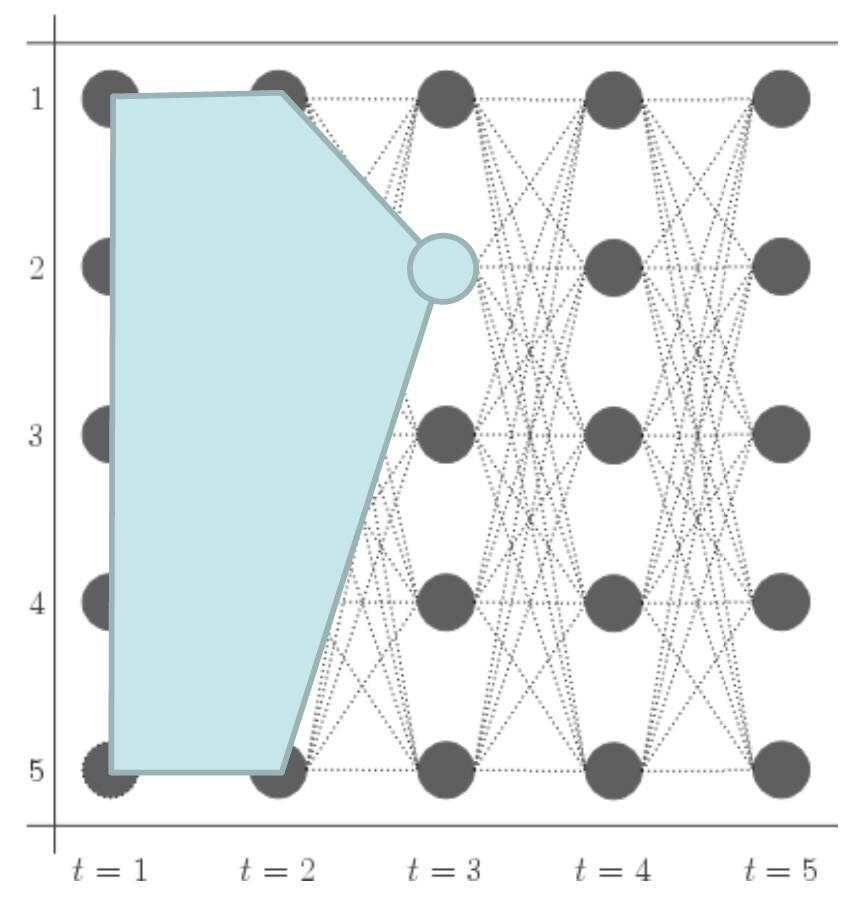
\includegraphics[scale=0.4]{images/forward.png}
        \end{center}

        Denote $\alpha_t(s_t)$ as sum of the unnormalized conditional probabilities ending at $s_t$ up to time $t$. For example, in the figure above, the shaded part refers to $\alpha_3(2)$, which is the sum of the unnormalized conditional probabilities ending at $s_3 = 2$ up to time $t = 3$. Particularly, the initial should be $\alpha_1(s_1) = \exp(\phi_e(s, 1, \mathbf{x}))$ in our CRF.

        Please write the recurrence formula for $\alpha_t(s_t)$ by using $\alpha_{t-1}(s_{t-1})$, $\phi_e$ and $\phi_t$.
        
        Given a sequence with length of $N$, write the relationship between $Z$ and $\alpha$.
        
        In practice, however, we usually use log-probability instead. By defining $\gamma_t(s_t) = \log \alpha_t(s_t)$, please write the recurrence formula for $\gamma_t(s_t)$ by using $\gamma_{t-1}(s_{t-1})$, $\phi_e$ and $\phi_t$, and show your work.
        
        \end{enumerate}

\end{document}